\documentclass[slidestop,compress,mathserif, aspectratio = 169, 9pt]{beamer}
\usecolortheme{seagull} % Beamer color theme
\useinnertheme{rectangles}
\usepackage[round]{natbib}
\usepackage{bibentry}
\usepackage{graphicx}
\usepackage{epigraph}
\usepackage{makeidx}
\usepackage[]{amsmath}
\usepackage[]{amssymb}
\usepackage{color}
\usepackage{pict2e}
\usepackage{algorithm2e}
\usepackage[ngerman]{babel}
\usepackage{tikz}
\usetikzlibrary{mindmap}
\usepackage{multirow}
\usepackage[utf8]{inputenc}
\usepackage{multimedia}
\usepackage{xcolor}
\usepackage{keyval}
\usepgfmodule{shapes}
\usepackage{pgfplots}
\usepackage{sansmath}
\usepackage{pgfgantt}
\usetikzlibrary{arrows}
\usepackage{colortbl}
\usepackage{array}
\usepackage{transparent}
\usepackage{txfonts}
\usepackage{eurosym}

\graphicspath{{../../../Vorlesungen/figures/}{./}}

\makeatletter
\tikzset{
  base/.is choice,
  base/top/.code={\let\vbox\vtop},
  base/bottom/.code={\def\pgfutil@minipage[t]{\minipage[b]}},
  % base/bottom/.code={}, % for plain TeX
}
\makeatother


\definecolor{mint}{rgb}{0,172,177}

 \pgfplotsset{width=7cm, height = 7cm}

 \setbeamertemplate{section page}
{
    \begin{centering}
    \vspace{2cm}
    \begin{beamercolorbox}[sep=12pt,center]{part title}
    \usebeamerfont{title}\insertsection\par
    \end{beamercolorbox}
    \end{centering}
}



\begin{document}

\newcommand{\source}[1]{\rotatebox{90}{\tiny \color{gray} #1}}

\newcommand{\done}{${\color{teal}\checkmark}$}

%% Formalia
\title{\color{white}\textbf{Bahningenieurwesen dual studieren}}
\subtitle{\color{white}\textbf{Entwurf Curriculum}}
\author[Jochim, Pfaff]{\color{white}\textbf{Prof. Dr.-Ing. Haldor Jochim, Prof. Dr. Raphael Pfaff}}
\institute[FH Aachen]{\color{white}\textbf{Fachhochschule Aachen}}
\date{}
\logo{\put(-18, 170){\includegraphics[width=1.4cm]{logoR}}}



{
\usebackgroundtemplate{\transparent{0.4}\includegraphics[width= \paperwidth]{EmmaCastle.jpg}}
\frame{\titlepage}

\usebackgroundtemplate{}

\section{\"Ubersicht}
\frame{\sectionpage}
\frame{\frametitle{\"Ubersicht Studienverlauf}
\framesubtitle{}
%\vspace{cm}
\begin{center}
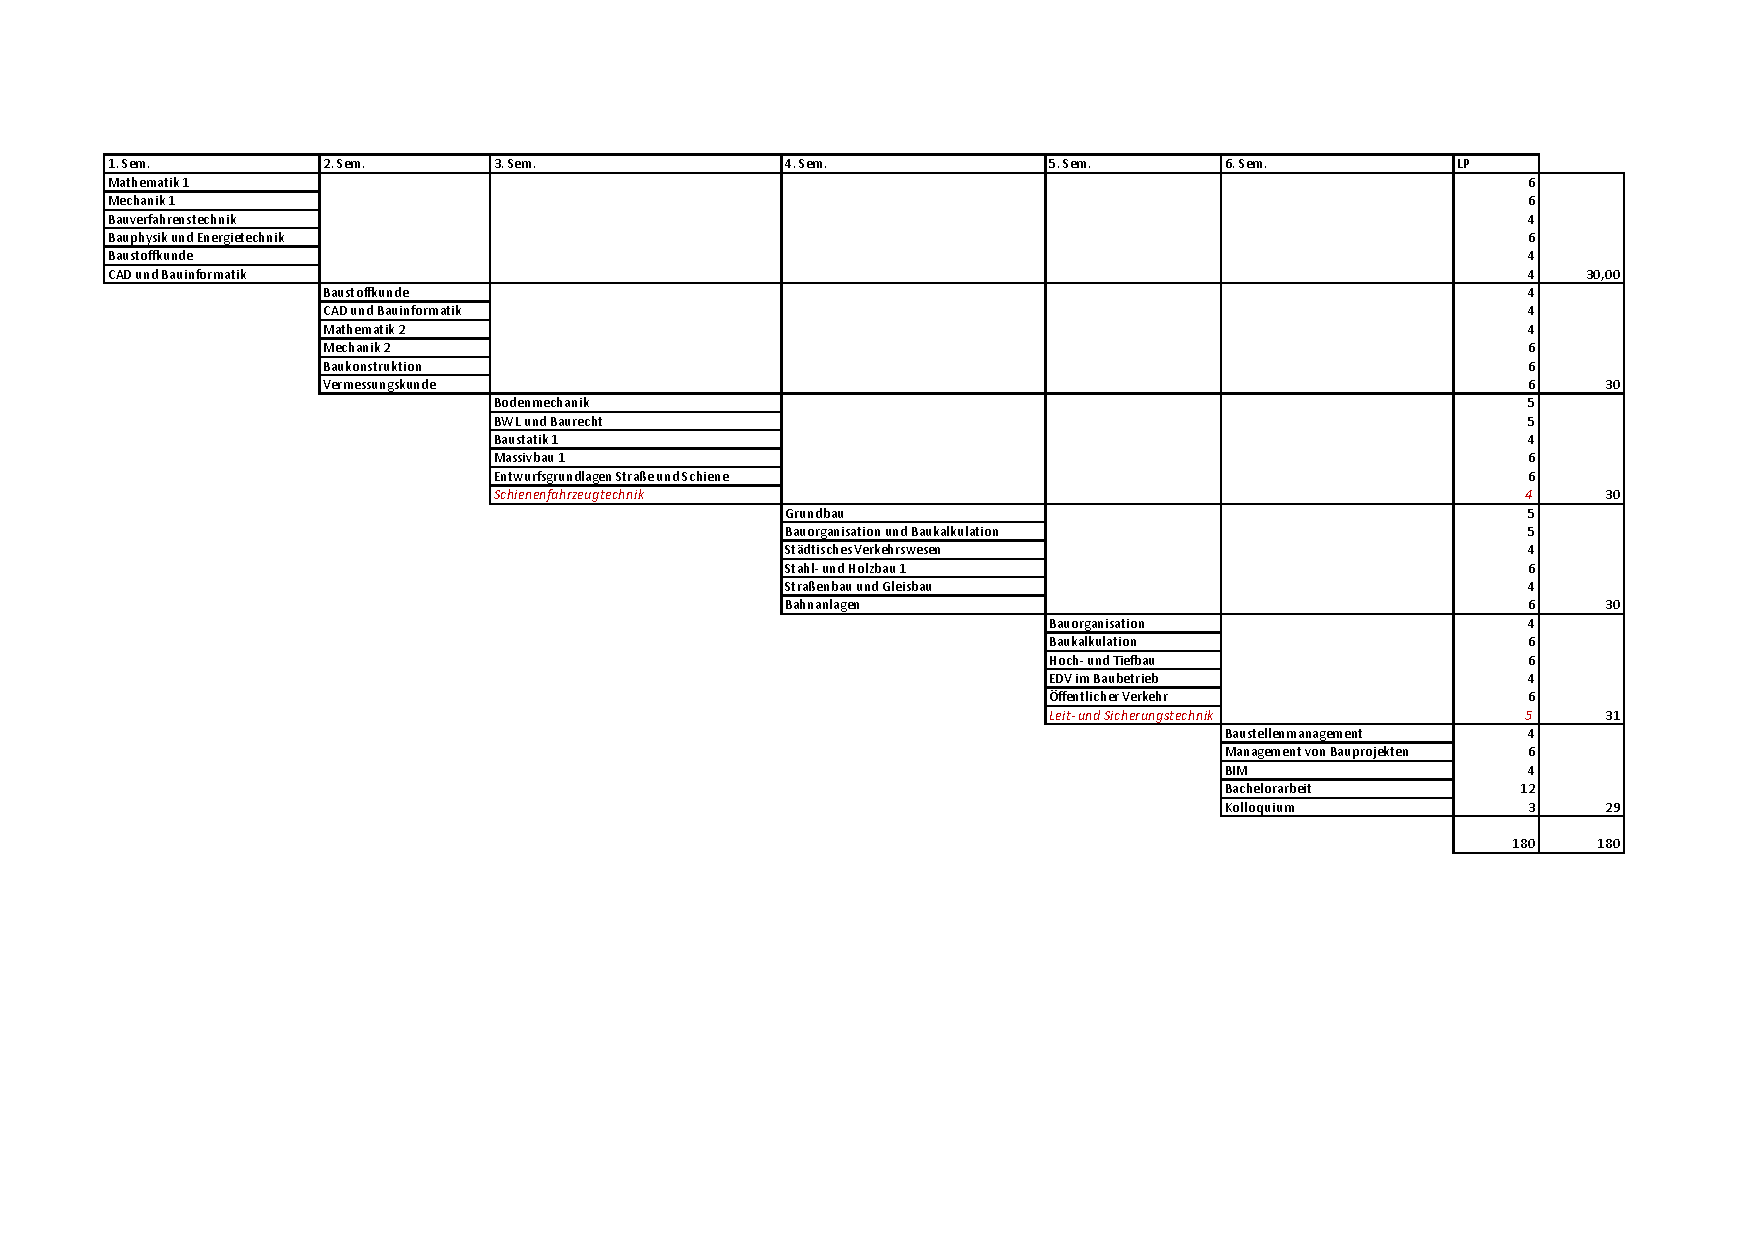
\includegraphics[width = \textwidth]{bahntechnik}
\end{center}
}

\section{Lernziele und Inhalte}
\frame{\sectionpage 
\centering Achtung: Die Lernziele bzw. Inhalte werden verk\"urzt dargestellt.}
}
%%%%%%%%%%%%%%% 1. Semester

\frame{\frametitle{Studieneingangsphase}
\framesubtitle{1. Semester (30 CP)}
\begin{columns}[t] 
     \begin{column}[T]{4.5cm} 
     Mathematik 1 (6 CP)
     	\begin{itemize}
     	\item Lineare Algebra und lineare Gleichungssysteme
     	\item Funktionentheorie
     	\item Grenzwertbestimmungen
     	\item Differentialrechnung
     	\end{itemize}
     \end{column}
     	\begin{column}[T]{4.5cm} 
	Mechanik 1 (6 CP)
     	\begin{itemize}
     	\item Zentrale und Allgemeine Kräftegruppen
     	\item Gleichgewicht ebener und räumlicher Körper
     	\item Schnittgrößenermittlung
     	\item Fachwerke
     	\item Reibung
     	\end{itemize}
     \end{column}
     \begin{column}[T]{4.5cm} 
     Bauverfahrenstechnik (4 CP)
     	\begin{itemize}
     	\item Baumaschinen 
	\item Baustelleneinrichtung
	\item Leistungsberechnung
	\item Auswahl Bauverfahren
     	\end{itemize}
     \end{column}
 \end{columns}
 
 \vspace{.5cm}
 
 \begin{columns}[t] 
     \begin{column}[T]{4.5cm} 
     Bauphysik (6 CP)
     	\begin{itemize}
%     	\item Physikalisches Grundlagenwissen 
	\item Wärmeschutz
	\item Energietechnik 
	\item Nutzung erneuerbarer Energien 
%	\item Europäische Verordnungen und Normen 
	\item Smart Building 
     	\end{itemize}
     \end{column}
     	\begin{column}[T]{4.5cm} 
	Baustoffkunde (4 CP)
     	\begin{itemize}
     	\item Rohstoffe und Verfahren
	\item Mechanischen, physikalische und chemische Eigenschaften 
	\item Anforderungs- und Prüfnormen
	 \end{itemize}
     \end{column}
     \begin{column}[T]{4.5cm} 
     CAD und Bauinformatik (4 CP)
     	\begin{itemize}
	\item Computer gestütztes Zeichnen und Planen (CAD, BIM)
	\item Tabellenkalkulation
	\item Textverarbeitung
	\item Programmieren
     	\end{itemize}
     \end{column}
 \end{columns}

}
%%%%%%%%%%%%%%% 2. Semester


\frame{\frametitle{Studieneingangsphase}
\framesubtitle{2. Semester (30 CP) (teils Fortsetzung zweisemestriger Module)}
\begin{columns}[t] 
     \begin{column}[T]{4.5cm} 
     Mathematik 2 (4 CP)
     	\begin{itemize}
     	\item Integralrechnung
	\item Vektorrechnung
	\item  Matrizenrechnung Gleichungssysteme
	\item Diskussion von Funktionen mehrerer Veränderlicher
	\item Gewöhnliche Differentialgleichungen
     	\end{itemize}
     \end{column}
     	\begin{column}[T]{4.5cm} 
	Mechanik 2 (6 CP)
     	\begin{itemize}
     	\item Spannungen und Dehnungen
	\item Verformungsbetrachtungen
	\item Ebener und räumlicher Spannungs- und Verzerrungszustand
	%\item Spannungen und Verformungen infolge Querkraft und Torsion
	\end{itemize}
     \end{column}
     \begin{column}[T]{4.5cm} 
     Baukonstruktion (6 CP)
     	\begin{itemize}
     	\item Sicherheitskonzept, Bauordnung
	%\item Elemente der Tragwerksplanung, Einwirkungen
	\item Gründungen/Abdichtung
	\item Konstruktionsprinzipien und Entwerfen im Betonbau
	\item Konstruktionsprinzipien im Stahlbau
     	\end{itemize}
     \end{column}
 \end{columns}
 
 \vspace{.5cm}
 
 \begin{columns}[t] 
     \begin{column}[T]{4.5cm} 
     Baustoffkunde (4 CP)
     	\begin{itemize}
     	\item Rohstoffe und Verfahren
	\item Mechanischen, physikalische und chemische Eigenschaften 
	\item Anforderungs- und Prüfnormen
	 \end{itemize}
     \end{column}
     	\begin{column}[T]{4.5cm} 
	Vermessungskunde (6 CP)
     	\begin{itemize}
     	\item Vermessungstätigkeiten durchf\"uhren
	\item Vermessungsleistungen werten
     	\end{itemize}
     \end{column}
     \begin{column}[T]{4.5cm} 
     CAD und Bauinformatik (4 CP)
     	\begin{itemize}
     	\item Computer gestütztes Zeichnen und Planen (CAD, BIM)
	\item Tabellenkalkulation
	\item Textverarbeitung
	\item Programmieren
     	\end{itemize}
     \end{column}
 \end{columns}

}

%%%%%%%%%%%%%%% 3. Semester


\frame{\frametitle{Studieneingangsphase}
\framesubtitle{3. Semester (30 CP)}
\begin{columns}[t] 
     \begin{column}[T]{4.5cm} 
     Bodenmechanik (5 CP)
     	\begin{itemize}
     	\item Ingenieurgeologische Grundlagen
	\item Bodenarten und Kenngrößen
	\item  Untersuchungsverfahren
	\item Boden als Baustoff
%	\item  WechselwirkungBauwerk -Baugrund
     	\end{itemize}
     \end{column}
     	\begin{column}[T]{4.5cm} 
	BWL und Baurecht (5 CP)
     	\begin{itemize}
     	\item Rechtsprechung bei öffentlichen Aufträgen
	\item Vergabemanagement und Vergabevorschriften
%	\item Erstellung von Angeboten als Bieter in Vergabeverfahren
	\item Vergabetaktik von Auftragnehmer und Auftraggeber
     	\end{itemize}
     \end{column}
     \begin{column}[T]{4.5cm} 
     Baustatik (4 CP)
     	\begin{itemize}
     	\item Grundsätzliche Abbildungsmöglichkeiten
	\item Weggrößenmethode
	\item Statische Berechnungen des Hochbaus und konstruktiven Ingenieurbaus 
     	\end{itemize}
     \end{column}
 \end{columns}
 
 \vspace{.5cm}
 
 \begin{columns}[t] 
     \begin{column}[T]{4.5cm} 
     Entwurfsgrundlagen Stra{\ss}e/Schiene (6 CP)
     	\begin{itemize}
	\item Ableitung der Trassierungsregeln für Schienenbahnen% aus Sicherheits-, Instandhaltungs- und Qualitätsaspekten
	\item Umgang mit der planerischen Flexibilität
	\item Grundlagen Betrieb des Schienenverkehrs% (exemplarisch) 
     	\end{itemize}
     \end{column}
     	\begin{column}[T]{4.5cm} 
	Massivbau 1 (6 CP)
%     	\begin{itemize}
%     	\item  Umgang mit technischer Literatur
%	\item Übung berufstypischer Alltagssituationen
%	\item Präsentationen
%	\item Erweiterung des technischen Wortschatzes
%     	\end{itemize}
     \end{column}
     \begin{column}[T]{4.5cm} 
     Schienenfahrzeugtechnik (4 CP)
\begin{itemize}
     	\item Grundlagen des Systems Schienenfahrzeug
	\item Anforderungen an Schienenfahrzeuge
	\item Spurführung und Zugdynamik
	\item Fahrzeug- und Drehgestellkonstruktion
	\end{itemize}
     \end{column}
 \end{columns}

}

%%%%%%%%%%%%%%% 4. Semester


\frame{\frametitle{Vertiefungsstudium}
\framesubtitle{4. Semester (32 CP)}
\begin{columns}[t] 
     \begin{column}[T]{4.5cm} 
     Stra{\ss}enbau und Gleisbau (4 CP)
     	\begin{itemize}
     	\item Gleisunterbau 
	\item  Schotterbett und Feste Fahrbahn
	 \item  Baubetriebsplanung
 	\item  Erhaltungs- und Unterhaltungsmanagement
     	\end{itemize}
     \end{column}
     	\begin{column}[T]{4.5cm} 
	Grundbau (5 CP)
     	\begin{itemize}
     	\item Gründungen, Baugruben und Böschungen/Geländesprüngen nach Eurocode 7
	\item Nachweiskonzepte für Grenzzustand
     	\end{itemize}
     \end{column}
     \begin{column}[T]{4.5cm} 
     Bauorganisation (5 CP)
     	\begin{itemize}
     	\item Ausschreibungs-, Vergabe- und Vertragswesen
	\item Bauzeitenplanung
 	\item Bauvorbereitung
	\item Arbeitssicherheit, Unfallverhütung
     	\end{itemize}
     \end{column}
 \end{columns}
 
 \vspace{.5cm}
 
 \begin{columns}[t] 
     \begin{column}[T]{4.5cm} 
     St\"adtisches Verkehrswesen (4 CP)
%     	\begin{itemize}
%     	\item Stromkreise (Gleich- und Wechselstrom) 
%	\item Symmetrische Last am Drehstromnetz 
%	\item Komplexe Wechselstromrechnung
%	\item Elektrische Maschinen
%     	\end{itemize}
     \end{column}
     	\begin{column}[T]{4.5cm} 
	Stahl- und Holzbau 1 (6 CP)
%     	\begin{itemize}
%     	\item Grundlagen Eisenbahnbetrieb
%	\item Grundlagen Fahrzeuge
%	\item Grundagen LST
%	\item Gesch\"aftmodelle im Eisenbahnbereich
%     	\end{itemize}
     \end{column}
     \begin{column}[T]{4.5cm} 
     Bahnanlagen (6 CP)
     	\begin{itemize}
     	\item Trassierung
     	\item Gestaltung von Knoten
     	\item Gleisbau
%     	\item Grundlagen der Sicherungstechnik (mit Labor)
     	\item Grundlagen des Fahrplanwesens
%     	\item Organisation des Schienenverkehrs
%     	\item Öffentlicher Nahverkehr (Grundlagen)
     	\end{itemize}
     \end{column}
 \end{columns}

}

%%%%%%%%%%%%%%% 5. Semester


\frame{\frametitle{Vertiefungsstudium}
\framesubtitle{5. Semester (31 CP)}
\begin{columns}[t] 
     \begin{column}[T]{6cm} 
     \"Offentlicher Verkehr (6 CP)
     	\begin{itemize}
     	\item Lösung von Planungsproblemen
	\item Infrastruktur und Management des öffentlichen Verkehrs
	\item Gesetzliche Grundlagen
	\item Wirtschaftlichkeit und Finanzierung
	\item Verkehrswirtschaft
     	\end{itemize}
     \end{column}
     	\begin{column}[T]{6cm} 
	Bauorganisation (4 CP)\\
	Baukalkulation (6 CP)\\
	Hoch- und Tiefbau (6 CP)\\
	EDV im Baubetrieb (4 CP)\\
%     	\begin{itemize}
%     	\item Wirtschaftlichkeit im Lebenszyklus
%	\item Qualitätsmanagement
%	\item Instandhaltungsstrategien
%	\item Zulassung nach EBO 
%	\item  Sicherheitsnachweise
%     	\end{itemize}
     \end{column}
     
  \end{columns}
 
 \vspace{.5cm}
 
 \begin{columns}[t] 
     \begin{column}[T]{6cm} 
     Leit- und Sicherheitstechnik (6 CP)
     	\begin{itemize}
     	\item Fahrwegssicherung und –steuerung
	\item Stellwerks- und Signalbauformen
	\item Zugleit- und Sicherungstechnik
	\item ERTMS/ETCS 
	\item Führen von Zügen im Simulator
     	\end{itemize}
     \end{column}

     \begin{column}[T]{6cm} 
     Schienenfahrzeugtechnik 1 (6 CP)
     	\begin{itemize}
     	\item Grundlagen des Systems Schienenfahrzeug
	\item Anforderungen an Schienenfahrzeuge
	\item Spurführung und Zugdynamik
	\item Fahrzeug- und Drehgestellkonstruktion
	\end{itemize}
     \end{column}
%     	\begin{column}[T]{4.5cm} 
%	BWL u. Technik der Eisenbahnen (6 CP)
%     	\begin{itemize}
%     	\item 
%     	\end{itemize}
%     \end{column}
%     \begin{column}[T]{4.5cm} 
%     Bahnanlagen (6 CP)
%     	\begin{itemize}
%     	\item Trassierung
%     	\item Gestaltung von Knoten
%     	\item Gleisbau
%%     	\item Grundlagen der Sicherungstechnik (mit Labor)
%     	\item Grundlagen des Fahrplanwesens
%%     	\item Organisation des Schienenverkehrs
%%     	\item Öffentlicher Nahverkehr (Grundlagen)
%     	\end{itemize}
%     \end{column}
 \end{columns}
}

%%%%%%%%%%%%%%% 6. Semester

\frame{\frametitle{Vertiefungsstudium}
\framesubtitle{6. Semester (29 CP)}
\begin{columns}[t] 
     \begin{column}[T]{6cm} 
     Baustellenmanagement (4 CP)\\
     Management von Bauprojekten (6 CP) \\
     BIM (4 CP)
     \end{column}
     \begin{column}[T]{6cm} 
     Bachelorarbeit mit Kolloquium (15 CP)
%     	\begin{itemize}
%     	\item 
%     	\end{itemize}
     \end{column}
 \end{columns}
 }


{
\usebackgroundtemplate{\transparent{0.4}\includegraphics[width= 1.45\paperwidth]{Lecker}}
\centering
\frame{\frametitle{Let's put awesome back into railways!}
\begin{tikzpicture}
 \path (0,0) -- (0cm,-7.5cm) node[rectangle, fill = white, opacity = 0.5, text opacity = 1] {Prof. Dr. Raphael Pfaff $\cdot$
			pfaff@fh-aachen.de $\cdot$
	+49-151-70052454 $\cdot$
		www.r10f.com};
\end{tikzpicture}

}
\end{document}
